\documentclass{beamer}
\usetheme{Marburg}
\title{The Code That Never Ran: Modeling Attacks on Speculative Evaluation}
\author{Craig Disselkoen \and Radha Jagadeesan \and Alan Jeffrey \and James Riely}

\definecolor{bottle}{rgb}{0,0.45,0.35}
\setbeamercolor{sidebar}{bg=bottle}
\setbeamercolor{frametitle}{fg=bottle}
\setbeamercolor{section in toc}{fg=bottle!50!black}
\setbeamercolor{author in sidebar}{fg=bottle!50!white}
\setbeamercolor{itemize item}{fg=bottle}
\setbeamertemplate{sidebar canvas right}[vertical shading][top=black,bottom=bottle]

\begin{document}

\begin{frame}[plain]
  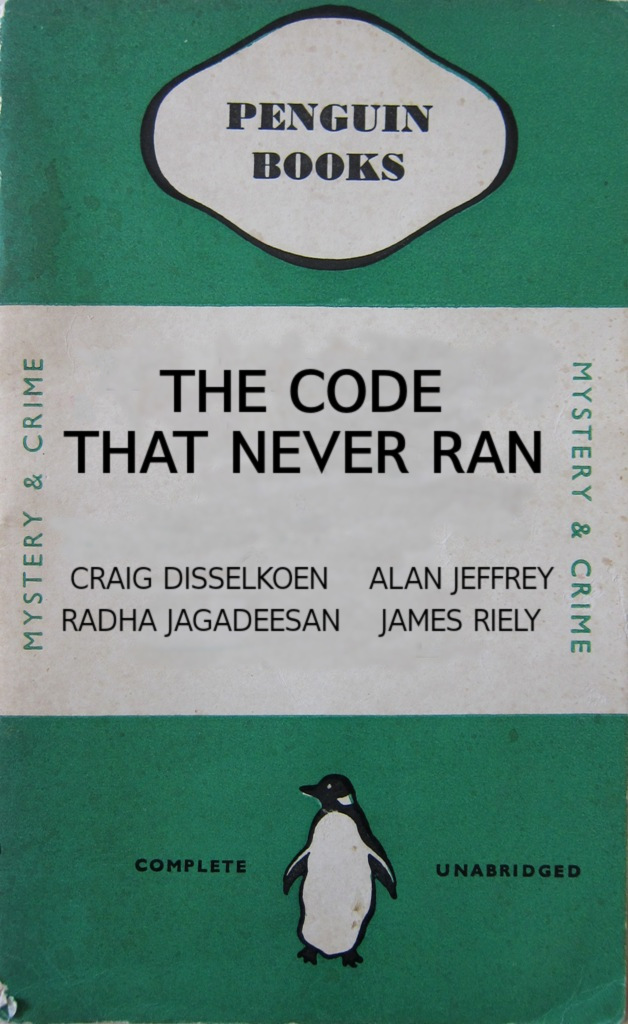
\includegraphics[height=.9\textheight]{green-penguin.jpg}
  \begin{minipage}[b][.9\textheight]{.66\textwidth}\raggedleft
    A classic locked-room mystery.\\
    Eve was in the false branch of a conditional the whole time,\\
    \emph{how could she do it}?

    \vss

    \tiny
    
\includegraphics[height=1.5ex]{cc-by-88x31.png}~Creative Commons Attribution-ShareAlike 4.0

    Mozilla Research \textbar~DePaul University \textbar~U.~California San Diego
  \end{minipage}
\end{frame}

\section{Introduction}
\begin{frame}{Overview}
  \begin{quotation}
  \tableofcontents
  \end{quotation}
\end{frame}

\begin{frame}[fragile]
  \frametitle{Why? Spectre!}

  {\fboxrule=1ex\fboxsep=0pt\fbox{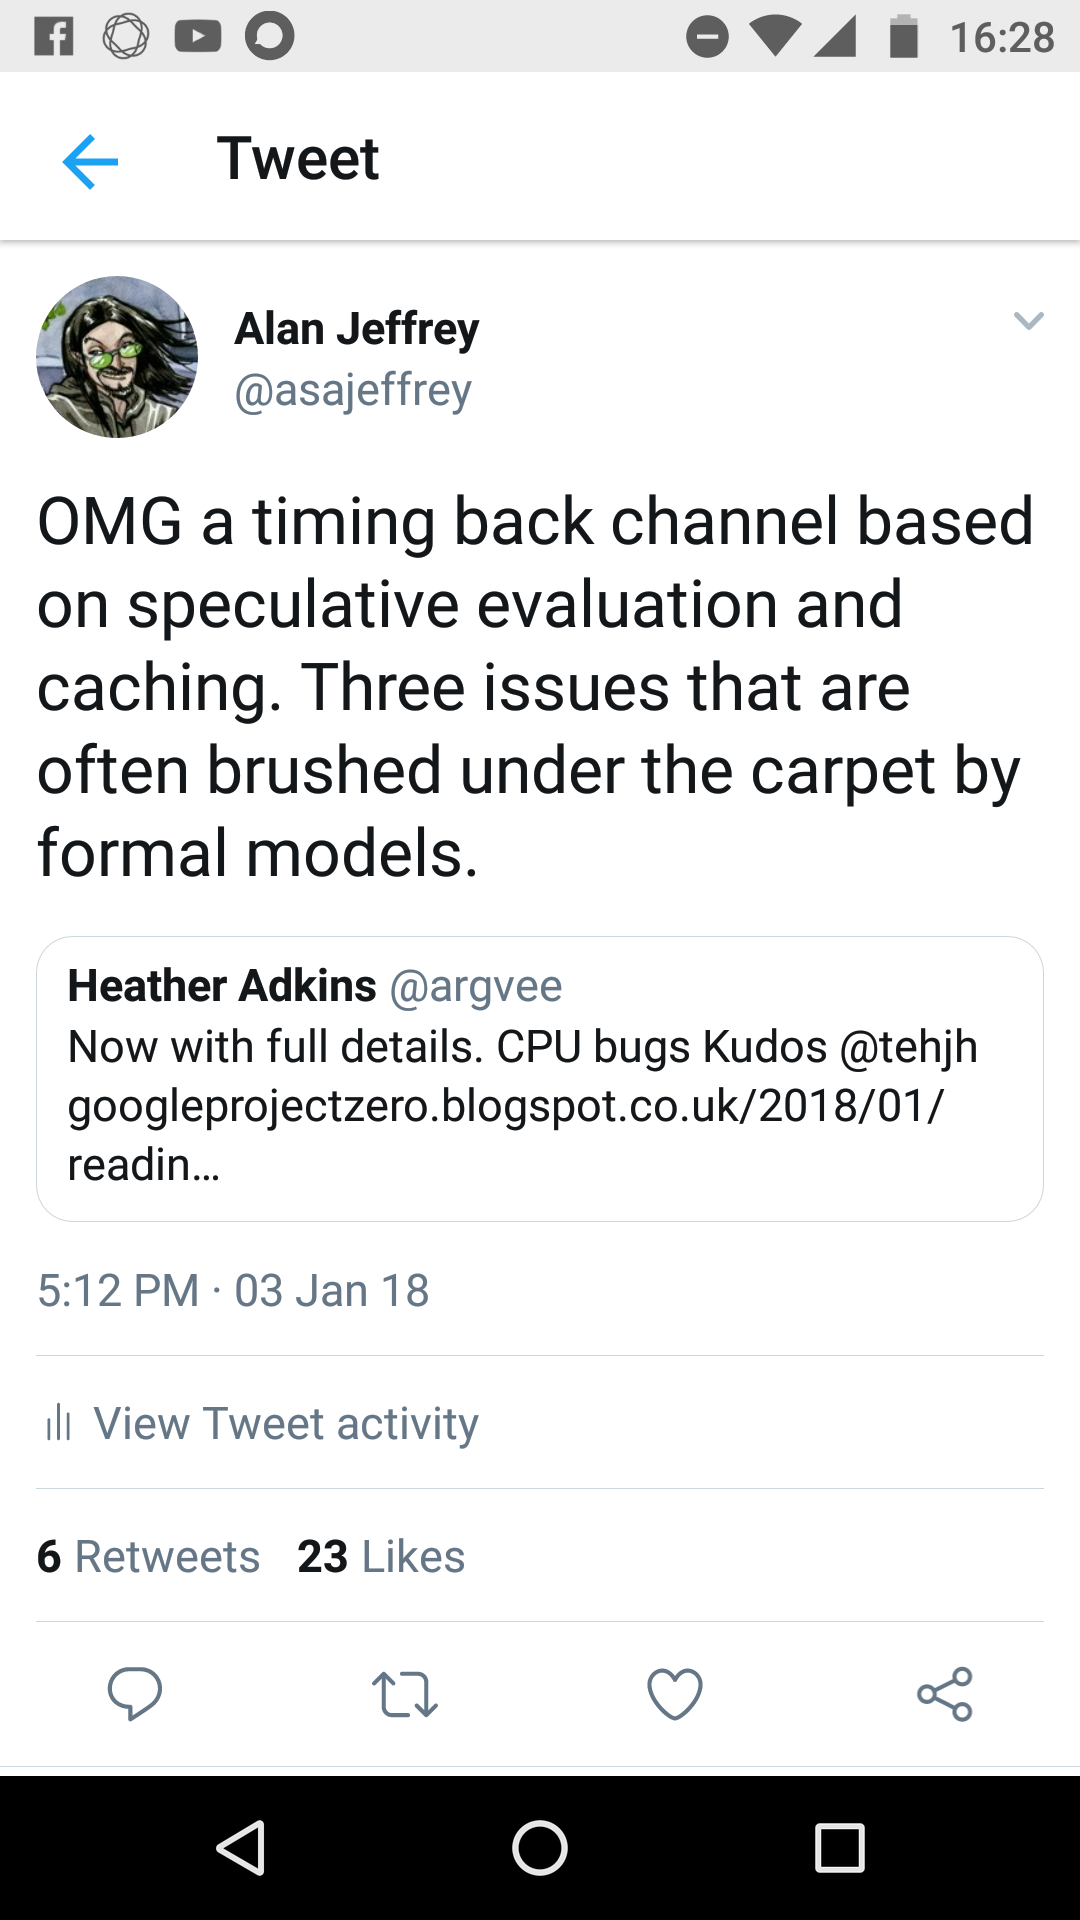
\includegraphics[height=.8\textheight]{omg-tweet.png}}}\quad\pause
  \begin{minipage}[b]{.45\textwidth}\raggedright
    Attacks bypass dynamic security checks:

\begin{verbatim}
if (canReadSecret) {
  doStuffWith(SECRET);
}
\end{verbatim}

    Information flow from \verb|SECRET|
    even though \verb|canReadSecret| is false.
    \bigskip

    Most formal models ignore code in branches
    that aren't taken.

    \bigskip
  \end{minipage}
\end{frame}

\begin{frame}
  \frametitle{Models that include speculation?}

  There are some models that include speculation\\
  \emph{relaxed memory models}:

  \begin{itemize}\footnotesize
  \item \emph{The Java Memory Model}\\
    Manson, Pugh and Adve, 2005.
  \item \emph{Generative Operational Semantics for Relaxed Memory Models}\\
    Jagadeesan, Pitcher and Riely, 2010.
  \item \emph{A promising semantics for relaxed-memory concurrency}\\
    Kang, Hur, Lahav, Vafeiadis and Dreyer, 2017.
  \end{itemize}

  \pause
  \emph{Question}: is there a simple model similar to
  those of relaxed memory, that can model speculation?
\end{frame}

\begin{frame}
  \frametitle{Information flow attacks on speculation}
  Speculation happens in many places:
  \begin{itemize}\footnotesize
  \item \emph{Speculation in hardware} (branch prediction,\ldots) \\
    \onslide<2->{Attacked by Spectre (Kocher \emph{et al.}~2019).}
  \item \emph{Transactions} (transactional memory,\ldots)\\
    \onslide<2->{Attacked by Prime+Abort (Disselokoen \emph{et al.}~2017).}
  \item \emph{Relaxed memory} (compiler optimizations,\ldots)\\
    \onslide<2->{No known attacks.}
  \end{itemize}
  
  \pause
  \emph{Question}: are there information flow attacks against
  compiler optimizations?
\end{frame}

\begin{frame}
  \frametitle{Contributions}
  \begin{itemize}\footnotesize
  \item A simple compositional model.
  \item Examples.
  \item Attacks (including a new attack on relaxed memory).
  \item Experiments (testing practicality of new attacks).
  \end{itemize}
\end{frame}

\section{Model}
\begin{frame}
  \frametitle{Model goes here}
\end{frame}

\section{Examples}
\begin{frame}
  \frametitle{Examples go here}
\end{frame}

\section{Attacks}
\begin{frame}
  \frametitle{Information flow attacks go here}
\end{frame}

\section{Experiments}
\begin{frame}
  \frametitle{Implementing the new attacks}
\end{frame}

\section{Conclusions}
\begin{frame}
  \frametitle{Outro goes here}
\end{frame}

\end{document}
